\section{Applied Theory}
\subsection{Definitions}
\index{acoustic feedback}\index{artifact}\index{howling}\index{sound reinforcement systems}
When most people talk about acoustic feedback they normally mean the unpleasant howling that can occur in sound reinforcement systems, technically this is wrong. Feedback is the mechanism of unwanted acoustic coupling between the speaker and the microphone, not the actual sound produced (called the howling). The unpleasant howling is called an \textit{artifact} and is but one of the artifacts that can occur as an result of acoustic feedback.

\subsection{Mathematical representation}
\index{mathematical models}
This representation of the problem is based on \cite{van_waterschoot_fifty_2011}. 

\index{state space model}
State space model can be seen from Figure \ref{feedmodel}. This is a model of $S$ sources, $S$ microphones and $L$ speakers.
\begin{figure}[H]
    \begin{center}
        % Graphic for TeX using PGF
% Title: /home/hvatum/skole/eit/Prosjektrapport/feed_model.dia
% Creator: Dia v0.97.2
% CreationDate: Fri Apr 26 09:10:36 2013
% For: hvatum
% \usepackage{tikz}
% The following commands are not supported in PSTricks at present
% We define them conditionally, so when they are implemented,
% this pgf file will use them.
\ifx\du\undefined
  \newlength{\du}
\fi
\setlength{\du}{6\unitlength}
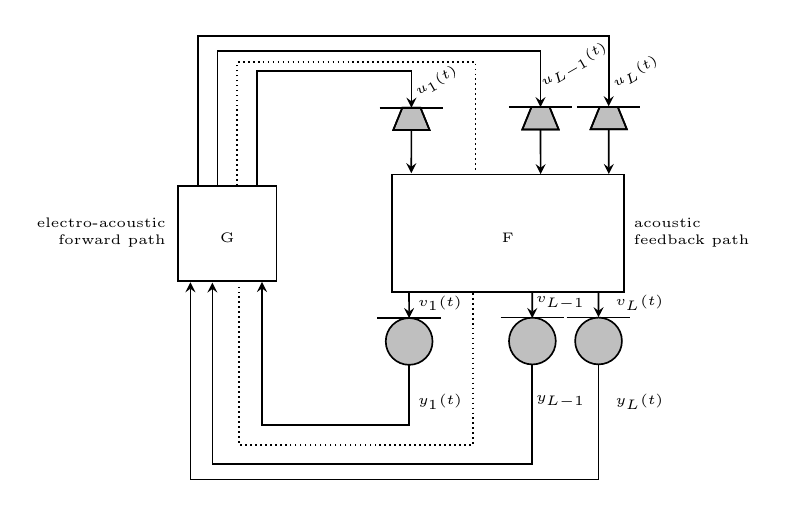
\begin{tikzpicture}
 \tikzstyle{every node}=[font=\tiny]
\pgftransformxscale{1.000000}
\pgftransformyscale{-1.000000}
\definecolor{dialinecolor}{rgb}{0.000000, 0.000000, 0.000000}
\pgfsetstrokecolor{dialinecolor}
\definecolor{dialinecolor}{rgb}{1.000000, 1.000000, 1.000000}
\pgfsetfillcolor{dialinecolor}
\pgfsetlinewidth{0.100000\du}
\pgfsetdash{}{0pt}
\pgfsetdash{}{0pt}
\pgfsetmiterjoin
\definecolor{dialinecolor}{rgb}{1.000000, 1.000000, 1.000000}
\pgfsetfillcolor{dialinecolor}
\fill (10.873900\du,8.392380\du)--(10.873900\du,14.113755\du)--(16.795057\du,14.113755\du)--(16.795057\du,8.392380\du)--cycle;
\definecolor{dialinecolor}{rgb}{0.000000, 0.000000, 0.000000}
\pgfsetstrokecolor{dialinecolor}
\draw (10.873900\du,8.392380\du)--(10.873900\du,14.113755\du)--(16.795057\du,14.113755\du)--(16.795057\du,8.392380\du)--cycle;
% setfont left to latex
\definecolor{dialinecolor}{rgb}{0.000000, 0.000000, 0.000000}
\pgfsetstrokecolor{dialinecolor}
\node at (13.834400\du,11.496850\du){G};
\pgfsetlinewidth{0.100000\du}
\pgfsetdash{}{0pt}
\pgfsetdash{}{0pt}
\pgfsetmiterjoin
\definecolor{dialinecolor}{rgb}{1.000000, 1.000000, 1.000000}
\pgfsetfillcolor{dialinecolor}
\fill (23.753300\du,7.715000\du)--(23.753300\du,14.791145\du)--(37.706643\du,14.791145\du)--(37.706643\du,7.715000\du)--cycle;
\definecolor{dialinecolor}{rgb}{0.000000, 0.000000, 0.000000}
\pgfsetstrokecolor{dialinecolor}
\draw (23.753300\du,7.715000\du)--(23.753300\du,14.791145\du)--(37.706643\du,14.791145\du)--(37.706643\du,7.715000\du)--cycle;
% setfont left to latex
\definecolor{dialinecolor}{rgb}{0.000000, 0.000000, 0.000000}
\pgfsetstrokecolor{dialinecolor}
\node at (30.730000\du,11.498100\du){F};
\pgfsetlinewidth{0.100000\du}
\pgfsetdash{}{0pt}
\pgfsetdash{}{0pt}
\pgfsetmiterjoin
\pgfsetbuttcap
{
\definecolor{dialinecolor}{rgb}{0.000000, 0.000000, 0.000000}
\pgfsetfillcolor{dialinecolor}
% was here!!!
\pgfsetarrowsend{stealth}
{\pgfsetcornersarced{\pgfpoint{0.000000\du}{0.000000\du}}\definecolor{dialinecolor}{rgb}{0.000000, 0.000000, 0.000000}
\pgfsetstrokecolor{dialinecolor}
\draw (12.058100\du,8.392380\du)--(12.058100\du,-0.621502\du)--(36.799274\du,-0.621502\du)--(36.799270\du,3.596142\du);
}}
\pgfsetlinewidth{0.100000\du}
\pgfsetdash{}{0pt}
\pgfsetdash{}{0pt}
\pgfsetbuttcap
{
\definecolor{dialinecolor}{rgb}{0.000000, 0.000000, 0.000000}
\pgfsetfillcolor{dialinecolor}
% was here!!!
\pgfsetarrowsend{stealth}
\definecolor{dialinecolor}{rgb}{0.000000, 0.000000, 0.000000}
\pgfsetstrokecolor{dialinecolor}
\draw (36.799300\du,4.987210\du)--(36.807600\du,7.678280\du);
}
\pgfsetlinewidth{0.100000\du}
\pgfsetdash{}{0pt}
\pgfsetdash{}{0pt}
\pgfsetbuttcap
\pgfsetmiterjoin
\pgfsetlinewidth{0.100000\du}
\pgfsetbuttcap
\pgfsetmiterjoin
\pgfsetdash{}{0pt}
\definecolor{dialinecolor}{rgb}{0.749020, 0.749020, 0.749020}
\pgfsetfillcolor{dialinecolor}
\fill (36.252085\du,3.641490\du)--(37.346454\du,3.641490\du)--(37.893638\du,4.987203\du)--(35.704900\du,4.987203\du)--cycle;
\definecolor{dialinecolor}{rgb}{0.000000, 0.000000, 0.000000}
\pgfsetstrokecolor{dialinecolor}
\draw (36.252085\du,3.641490\du)--(37.346454\du,3.641490\du)--(37.893638\du,4.987203\du)--(35.704900\du,4.987203\du)--cycle;
\pgfsetbuttcap
\pgfsetmiterjoin
\pgfsetdash{}{0pt}
\definecolor{dialinecolor}{rgb}{0.000000, 0.000000, 0.000000}
\pgfsetstrokecolor{dialinecolor}
\draw (36.252085\du,3.641490\du)--(37.346454\du,3.641490\du)--(37.893638\du,4.987203\du)--(35.704900\du,4.987203\du)--cycle;
\pgfsetlinewidth{0.100000\du}
\pgfsetdash{}{0pt}
\pgfsetdash{}{0pt}
\pgfsetbuttcap
{
\definecolor{dialinecolor}{rgb}{0.000000, 0.000000, 0.000000}
\pgfsetfillcolor{dialinecolor}
% was here!!!
\definecolor{dialinecolor}{rgb}{0.000000, 0.000000, 0.000000}
\pgfsetstrokecolor{dialinecolor}
\draw (34.888300\du,3.640380\du)--(38.704200\du,3.640380\du);
}
\pgfsetlinewidth{0.100000\du}
\pgfsetdash{}{0pt}
\pgfsetdash{}{0pt}
\pgfsetbuttcap
{
\definecolor{dialinecolor}{rgb}{0.000000, 0.000000, 0.000000}
\pgfsetfillcolor{dialinecolor}
% was here!!!
\definecolor{dialinecolor}{rgb}{0.000000, 0.000000, 0.000000}
\pgfsetstrokecolor{dialinecolor}
\draw (10.873900\du,8.392380\du)--(16.795000\du,8.392380\du);
}
\pgfsetlinewidth{0.100000\du}
\pgfsetdash{}{0pt}
\pgfsetdash{}{0pt}
\pgfsetmiterjoin
\pgfsetbuttcap
{
\definecolor{dialinecolor}{rgb}{0.000000, 0.000000, 0.000000}
\pgfsetfillcolor{dialinecolor}
% was here!!!
\pgfsetarrowsend{stealth}
{\pgfsetcornersarced{\pgfpoint{0.000000\du}{0.000000\du}}\definecolor{dialinecolor}{rgb}{0.000000, 0.000000, 0.000000}
\pgfsetstrokecolor{dialinecolor}
\draw (15.610800\du,8.392380\du)--(15.610800\du,1.487530\du)--(24.917000\du,1.487530\du)--(24.917000\du,3.686090\du);
}}
\pgfsetlinewidth{0.100000\du}
\pgfsetdash{}{0pt}
\pgfsetdash{}{0pt}
\pgfsetbuttcap
{
\definecolor{dialinecolor}{rgb}{0.000000, 0.000000, 0.000000}
\pgfsetfillcolor{dialinecolor}
% was here!!!
\pgfsetarrowsend{stealth}
\definecolor{dialinecolor}{rgb}{0.000000, 0.000000, 0.000000}
\pgfsetstrokecolor{dialinecolor}
\draw (24.917000\du,5.031800\du)--(24.909100\du,7.629670\du);
}
\pgfsetlinewidth{0.100000\du}
\pgfsetdash{}{0pt}
\pgfsetdash{}{0pt}
\pgfsetmiterjoin
\pgfsetbuttcap
{
\definecolor{dialinecolor}{rgb}{0.000000, 0.000000, 0.000000}
\pgfsetfillcolor{dialinecolor}
% was here!!!
\pgfsetarrowsend{stealth}
{\pgfsetcornersarced{\pgfpoint{0.000000\du}{0.000000\du}}\definecolor{dialinecolor}{rgb}{0.000000, 0.000000, 0.000000}
\pgfsetstrokecolor{dialinecolor}
\draw (13.242300\du,8.392380\du)--(13.242300\du,0.250649\du)--(32.691300\du,0.250649\du)--(32.691300\du,3.650940\du);
}}
\pgfsetlinewidth{0.100000\du}
\pgfsetdash{}{0pt}
\pgfsetdash{}{0pt}
\pgfsetbuttcap
{
\definecolor{dialinecolor}{rgb}{0.000000, 0.000000, 0.000000}
\pgfsetfillcolor{dialinecolor}
% was here!!!
\pgfsetarrowsend{stealth}
\definecolor{dialinecolor}{rgb}{0.000000, 0.000000, 0.000000}
\pgfsetstrokecolor{dialinecolor}
\draw (32.691300\du,4.996650\du)--(32.699600\du,7.687730\du);
}
\pgfsetlinewidth{0.100000\du}
\pgfsetdash{}{0pt}
\pgfsetdash{}{0pt}
\pgfsetbuttcap
\pgfsetmiterjoin
\pgfsetlinewidth{0.100000\du}
\pgfsetbuttcap
\pgfsetmiterjoin
\pgfsetdash{}{0pt}
\definecolor{dialinecolor}{rgb}{0.749020, 0.749020, 0.749020}
\pgfsetfillcolor{dialinecolor}
\fill (32.144185\du,3.650940\du)--(33.238554\du,3.650940\du)--(33.785738\du,4.996653\du)--(31.597000\du,4.996653\du)--cycle;
\definecolor{dialinecolor}{rgb}{0.000000, 0.000000, 0.000000}
\pgfsetstrokecolor{dialinecolor}
\draw (32.144185\du,3.650940\du)--(33.238554\du,3.650940\du)--(33.785738\du,4.996653\du)--(31.597000\du,4.996653\du)--cycle;
\pgfsetbuttcap
\pgfsetmiterjoin
\pgfsetdash{}{0pt}
\definecolor{dialinecolor}{rgb}{0.000000, 0.000000, 0.000000}
\pgfsetstrokecolor{dialinecolor}
\draw (32.144185\du,3.650940\du)--(33.238554\du,3.650940\du)--(33.785738\du,4.996653\du)--(31.597000\du,4.996653\du)--cycle;
\pgfsetlinewidth{0.100000\du}
\pgfsetdash{}{0pt}
\pgfsetdash{}{0pt}
\pgfsetbuttcap
{
\definecolor{dialinecolor}{rgb}{0.000000, 0.000000, 0.000000}
\pgfsetfillcolor{dialinecolor}
% was here!!!
\definecolor{dialinecolor}{rgb}{0.000000, 0.000000, 0.000000}
\pgfsetstrokecolor{dialinecolor}
\draw (30.780300\du,3.649820\du)--(34.596200\du,3.649820\du);
}
\pgfsetlinewidth{0.100000\du}
\pgfsetdash{{\pgflinewidth}{0.200000\du}}{0cm}
\pgfsetdash{{\pgflinewidth}{0.200000\du}}{0cm}
\pgfsetmiterjoin
\pgfsetbuttcap
{
\definecolor{dialinecolor}{rgb}{0.000000, 0.000000, 0.000000}
\pgfsetfillcolor{dialinecolor}
% was here!!!
{\pgfsetcornersarced{\pgfpoint{0.000000\du}{0.000000\du}}\definecolor{dialinecolor}{rgb}{0.000000, 0.000000, 0.000000}
\pgfsetstrokecolor{dialinecolor}
\draw (14.426600\du,8.392380\du)--(14.426600\du,0.934434\du)--(28.777600\du,0.934434\du)--(28.777600\du,7.593900\du);
}}
\pgfsetlinewidth{0.100000\du}
\pgfsetdash{}{0pt}
\pgfsetdash{}{0pt}
\pgfsetbuttcap
{
\definecolor{dialinecolor}{rgb}{0.000000, 0.000000, 0.000000}
\pgfsetfillcolor{dialinecolor}
% was here!!!
\pgfsetarrowsend{stealth}
\definecolor{dialinecolor}{rgb}{0.000000, 0.000000, 0.000000}
\pgfsetstrokecolor{dialinecolor}
\draw (36.186300\du,14.800800\du)--(36.184300\du,16.303500\du);
}
\pgfsetlinewidth{0.100000\du}
\pgfsetdash{}{0pt}
\pgfsetdash{}{0pt}
\pgfsetbuttcap
{
\definecolor{dialinecolor}{rgb}{0.000000, 0.000000, 0.000000}
\pgfsetfillcolor{dialinecolor}
% was here!!!
\pgfsetarrowsend{stealth}
\definecolor{dialinecolor}{rgb}{0.000000, 0.000000, 0.000000}
\pgfsetstrokecolor{dialinecolor}
\draw (24.774100\du,14.800800\du)--(24.780500\du,16.352900\du);
}
\pgfsetlinewidth{0.100000\du}
\pgfsetdash{}{0pt}
\pgfsetdash{}{0pt}
\pgfsetbuttcap
{
\definecolor{dialinecolor}{rgb}{0.000000, 0.000000, 0.000000}
\pgfsetfillcolor{dialinecolor}
% was here!!!
\pgfsetarrowsend{stealth}
\definecolor{dialinecolor}{rgb}{0.000000, 0.000000, 0.000000}
\pgfsetstrokecolor{dialinecolor}
\draw (32.195900\du,14.800800\du)--(32.192900\du,16.352900\du);
}
\pgfsetlinewidth{0.100000\du}
\pgfsetdash{{\pgflinewidth}{0.200000\du}}{0cm}
\pgfsetdash{{\pgflinewidth}{0.200000\du}}{0cm}
\pgfsetmiterjoin
\pgfsetbuttcap
{
\definecolor{dialinecolor}{rgb}{0.000000, 0.000000, 0.000000}
\pgfsetfillcolor{dialinecolor}
% was here!!!
{\pgfsetcornersarced{\pgfpoint{0.000000\du}{0.000000\du}}\definecolor{dialinecolor}{rgb}{0.000000, 0.000000, 0.000000}
\pgfsetstrokecolor{dialinecolor}
\draw (28.630000\du,14.841600\du)--(28.630000\du,24.006200\du)--(14.546000\du,24.006200\du)--(14.546000\du,14.256400\du);
}}
\pgfsetlinewidth{0.100000\du}
\pgfsetdash{}{0pt}
\pgfsetdash{}{0pt}
\pgfsetmiterjoin
\pgfsetbuttcap
{
\definecolor{dialinecolor}{rgb}{0.000000, 0.000000, 0.000000}
\pgfsetfillcolor{dialinecolor}
% was here!!!
\pgfsetarrowsend{stealth}
{\pgfsetcornersarced{\pgfpoint{0.000000\du}{0.000000\du}}\definecolor{dialinecolor}{rgb}{0.000000, 0.000000, 0.000000}
\pgfsetstrokecolor{dialinecolor}
\draw (32.192900\du,19.169900\du)--(32.192900\du,25.130100\du)--(12.931200\du,25.130100\du)--(12.931200\du,14.214400\du);
}}
\pgfsetlinewidth{0.100000\du}
\pgfsetdash{}{0pt}
\pgfsetdash{}{0pt}
\pgfsetmiterjoin
\pgfsetbuttcap
{
\definecolor{dialinecolor}{rgb}{0.000000, 0.000000, 0.000000}
\pgfsetfillcolor{dialinecolor}
% was here!!!
\pgfsetarrowsend{stealth}
{\pgfsetcornersarced{\pgfpoint{0.000000\du}{0.000000\du}}\definecolor{dialinecolor}{rgb}{0.000000, 0.000000, 0.000000}
\pgfsetstrokecolor{dialinecolor}
\draw (36.182400\du,19.169900\du)--(36.182400\du,26.084700\du)--(11.605400\du,26.084700\du)--(11.605400\du,14.196700\du);
}}
\pgfsetlinewidth{0.100000\du}
\pgfsetdash{}{0pt}
\pgfsetdash{}{0pt}
\pgfsetmiterjoin
\pgfsetbuttcap
{
\definecolor{dialinecolor}{rgb}{0.000000, 0.000000, 0.000000}
\pgfsetfillcolor{dialinecolor}
% was here!!!
\pgfsetarrowsend{stealth}
{\pgfsetcornersarced{\pgfpoint{0.000000\du}{0.000000\du}}\definecolor{dialinecolor}{rgb}{0.000000, 0.000000, 0.000000}
\pgfsetstrokecolor{dialinecolor}
\draw (24.780500\du,19.169900\du)--(24.780500\du,22.806200\du)--(15.918700\du,22.806200\du)--(15.918700\du,14.179000\du);
}}
% setfont left to latex
\definecolor{dialinecolor}{rgb}{0.000000, 0.000000, 0.000000}
\pgfsetstrokecolor{dialinecolor}
\node[anchor=west,rotate=30] at (24.716400\du,3.093200\du){$u_1(t)$};
\node[anchor=west,rotate=30] at (32.316400\du,2.593200\du){$u_{L-1}(t)$};
\node[anchor=west,rotate=30] at (36.616400\du,2.593200\du){$u_{L}(t)$};

\node[anchor=west] at (24.716400\du,15.453200\du){$v_1(t)$};
\node[anchor=west] at (31.816400\du,15.453200\du){$v_{L-1}$};
\node[anchor=west] at (36.616400\du,15.453200\du){$v_{L}(t)$};

\node[anchor=east] at (10.716400\du,10.593200\du){electro-acoustic};
\node[anchor=east] at (10.716400\du,11.693200\du){forward path};

\node[anchor=west] at (37.716400\du,10.593200\du){acoustic};
\node[anchor=west] at (37.716400\du,11.693200\du){feedback path};

% setfont left to latex
\definecolor{dialinecolor}{rgb}{0.000000, 0.000000, 0.000000}
\pgfsetstrokecolor{dialinecolor}
\node[anchor=west] at (24.716400\du,21.393200\du){$y_1(t)$};
\node[anchor=west] at (31.816400\du,21.393200\du){$y_{L-1}$};
\node[anchor=west] at (36.616400\du,21.393200\du){$y_{L}(t)$};
\pgfsetlinewidth{0.100000\du}
\pgfsetdash{}{0pt}
\pgfsetdash{}{0pt}
\pgfsetbuttcap
\pgfsetmiterjoin
\pgfsetlinewidth{0.100000\du}
\pgfsetbuttcap
\pgfsetmiterjoin
\pgfsetdash{}{0pt}
\definecolor{dialinecolor}{rgb}{0.749020, 0.749020, 0.749020}
\pgfsetfillcolor{dialinecolor}
\fill (24.369785\du,3.686090\du)--(25.464154\du,3.686090\du)--(26.011338\du,5.031803\du)--(23.822600\du,5.031803\du)--cycle;
\definecolor{dialinecolor}{rgb}{0.000000, 0.000000, 0.000000}
\pgfsetstrokecolor{dialinecolor}
\draw (24.369785\du,3.686090\du)--(25.464154\du,3.686090\du)--(26.011338\du,5.031803\du)--(23.822600\du,5.031803\du)--cycle;
\pgfsetbuttcap
\pgfsetmiterjoin
\pgfsetdash{}{0pt}
\definecolor{dialinecolor}{rgb}{0.000000, 0.000000, 0.000000}
\pgfsetstrokecolor{dialinecolor}
\draw (24.369785\du,3.686090\du)--(25.464154\du,3.686090\du)--(26.011338\du,5.031803\du)--(23.822600\du,5.031803\du)--cycle;
\pgfsetlinewidth{0.100000\du}
\pgfsetdash{}{0pt}
\pgfsetdash{}{0pt}
\pgfsetbuttcap
{
\definecolor{dialinecolor}{rgb}{0.000000, 0.000000, 0.000000}
\pgfsetfillcolor{dialinecolor}
% was here!!!
\definecolor{dialinecolor}{rgb}{0.000000, 0.000000, 0.000000}
\pgfsetstrokecolor{dialinecolor}
\draw (23.005900\du,3.684970\du)--(26.821900\du,3.684970\du);
}
\definecolor{dialinecolor}{rgb}{0.749020, 0.749020, 0.749020}
\pgfsetfillcolor{dialinecolor}
\pgfpathellipse{\pgfpoint{24.780481\du}{17.761381\du}}{\pgfpoint{1.408481\du}{0\du}}{\pgfpoint{0\du}{1.408481\du}}
\pgfusepath{fill}
\pgfsetlinewidth{0.100000\du}
\pgfsetdash{}{0pt}
\pgfsetdash{}{0pt}
\definecolor{dialinecolor}{rgb}{0.000000, 0.000000, 0.000000}
\pgfsetstrokecolor{dialinecolor}
\pgfpathellipse{\pgfpoint{24.780481\du}{17.761381\du}}{\pgfpoint{1.408481\du}{0\du}}{\pgfpoint{0\du}{1.408481\du}}
\pgfusepath{stroke}
\pgfsetlinewidth{0.100000\du}
\pgfsetdash{}{0pt}
\pgfsetdash{}{0pt}
\pgfsetbuttcap
{
\definecolor{dialinecolor}{rgb}{0.000000, 0.000000, 0.000000}
\pgfsetfillcolor{dialinecolor}
% was here!!!
\definecolor{dialinecolor}{rgb}{0.000000, 0.000000, 0.000000}
\pgfsetstrokecolor{dialinecolor}
\draw (22.864400\du,16.340900\du)--(26.680300\du,16.340900\du);
}
\definecolor{dialinecolor}{rgb}{0.749020, 0.749020, 0.749020}
\pgfsetfillcolor{dialinecolor}
\pgfpathellipse{\pgfpoint{32.202681\du}{17.738581\du}}{\pgfpoint{1.408481\du}{0\du}}{\pgfpoint{0\du}{1.408481\du}}
\pgfusepath{fill}
\pgfsetlinewidth{0.100000\du}
\pgfsetdash{}{0pt}
\pgfsetdash{}{0pt}
\definecolor{dialinecolor}{rgb}{0.000000, 0.000000, 0.000000}
\pgfsetstrokecolor{dialinecolor}
\pgfpathellipse{\pgfpoint{32.202681\du}{17.738581\du}}{\pgfpoint{1.408481\du}{0\du}}{\pgfpoint{0\du}{1.408481\du}}
\pgfusepath{stroke}
\pgfsetlinewidth{0.100000\du}
\pgfsetdash{}{0pt}
\pgfsetdash{}{0pt}
\pgfsetbuttcap
{
\definecolor{dialinecolor}{rgb}{0.000000, 0.000000, 0.000000}
\pgfsetfillcolor{dialinecolor}
% was here!!!
\definecolor{dialinecolor}{rgb}{0.000000, 0.000000, 0.000000}
\pgfsetstrokecolor{dialinecolor}
\draw (30.286600\du,16.318000\du)--(34.102500\du,16.318000\du);
}
\definecolor{dialinecolor}{rgb}{0.749020, 0.749020, 0.749020}
\pgfsetfillcolor{dialinecolor}
\pgfpathellipse{\pgfpoint{36.186481\du}{17.734181\du}}{\pgfpoint{1.408481\du}{0\du}}{\pgfpoint{0\du}{1.408481\du}}
\pgfusepath{fill}
\pgfsetlinewidth{0.100000\du}
\pgfsetdash{}{0pt}
\pgfsetdash{}{0pt}
\definecolor{dialinecolor}{rgb}{0.000000, 0.000000, 0.000000}
\pgfsetstrokecolor{dialinecolor}
\pgfpathellipse{\pgfpoint{36.186481\du}{17.734181\du}}{\pgfpoint{1.408481\du}{0\du}}{\pgfpoint{0\du}{1.408481\du}}
\pgfusepath{stroke}
\pgfsetlinewidth{0.100000\du}
\pgfsetdash{}{0pt}
\pgfsetdash{}{0pt}
\pgfsetbuttcap
{
\definecolor{dialinecolor}{rgb}{0.000000, 0.000000, 0.000000}
\pgfsetfillcolor{dialinecolor}
% was here!!!
\definecolor{dialinecolor}{rgb}{0.000000, 0.000000, 0.000000}
\pgfsetstrokecolor{dialinecolor}
\draw (34.270400\du,16.313600\du)--(38.086300\du,16.313600\du);
}
\end{tikzpicture}

    \end{center}
    \caption{Discrete-time model of a Sound reinforcement system}
    \label{feedmodel}
\end{figure} 
Mathematically this can be represented as:
\begin{eqnarray}
\mathbf{y}= \mathbf{F}(q,t)\mathbf{u}(t) + \mathbf{v}(t)\\
\mathbf{u} = \mathbf{G}[\mathbf{y}(t),t]
\end{eqnarray}
The source signal $\mathbf{v}_i(t)$, microphone signal $\mathbf{y}_i(t)$ and loudspeaker signal vectors $\mathbf{u}_j(t)$ are defined as: 
\begin{eqnarray}
\mathbf{v}(t) = [v_1(t) \ldots v_S]^T \\
\mathbf{y}(t) = [y_1(t) \ldots y_S]^T \\
\mathbf{u}(t) = [u_1(t) \ldots v_L]^T
\end{eqnarray}
The matrix $\mathbf{F}(q,t)$ is the multi channel acoustic \textit{feedback path}, $\mathbf{G}(\cdot,t)$ is the electroacoustic forward path characteristics or \textit{forward path}.

Between each loudspeaker-microphone pair $(i,j)$ there exists an acoustic coupling, this is modeled by the nth order acoustic feedback path transfer function:
\begin{equation}
	F_{ij}(q,t) = f_{ij}^{(0)}(t) + f_{ij}^{(1)}(t)q^{-1} + \ldots + f_{ij}^{(n_F)}(t)q^{-n_F}
\end{equation}
$q$ is the discrete time shift operator: $q^{-k}f(t) = f(t-k)$.

We can define the feedback path as a matrix of all the possible couplings:
\begin{eqnarray}
\mathbf{F}(q,t) =
\begin{bmatrix}
F_{11}(q,t) & \ldots & F_{1L}(q,t)\\
\vdots & \ldots & \vdots\\
F_{S1}(q,t) & \ldots & F_{SL}(q,t)
\end{bmatrix}
\end{eqnarray}
The acoustic feedback path model is linear, time varying and of finite order \cite{van_waterschoot_fifty_2011}.\\

The proposed solution simplifies this path by assuming a single speaker a single microphone, this is not a unreasonable assumption since most sound reinforcement systems for speech consists of two speakers and one microphone. The simplified version of the feedback path seems good enough to provide a proof of concept. The resulting model for both the feedback and feed-forward path can be seen as scalar.\\

\subsection{Two-stage NHS}
\index{Notch-filter}
\nomenclature{NHS}{Notch filter Howling Suppression} 
The method used in this system is the two-stage Notch filter based Howling Suppression (NHS), this is a simple and reliable method that is commonly used in howling prevention \cite{van_waterschoot_fifty_2011}. The figure \ref{NHS_overview} shows the overall conceptual structure of the method.

\begin{figure}[H]
\centering
\includegraphics[width=14cm]{description/Figures/Two-stage_NHS-2}
\caption{Two-stage NHS structure}
\label{NHS_overview}
\end{figure}

In this figure \ref{NHS_overview} $G$ is the transfer function of the electro-acoustical feed forward path, $F$ is the feedback path, and $H$ is an equalizer that consists of a bank of adjustable notch-filters. The signals are given by non-capital letters where $v(t)$ is the wanted audio signal from the person or instrument in front of the microphone, $y(t)$ is one frame of samples of this signal in the time plane, $D$ is a vector of frequencies where howling has been detected, $d(t)$ is the signal after it has been filtered though the adjustable bank of notch-filters, $u(t)$ is the output to the speaker(s), $x(t)$ is the unwanted feedback signal.\\
\\
\index{howling}\index{feedback loop}
The howling detection is designed to detect howling and return a vector of frequencies on which howling is detected. These frequencies will correspond to a notch-filter in the equalizer, reducing the gain on these frequencies. Hopefully this reduction in frequency gain is enough to break the positive feedback loop end stop the howling. \\
\\
\index{power spectrum}
The howling detection scheme looks at the power spectrum of the signal and picks out peaks, these peaks are subjected to several tests. Peaks are tested for discriminating features between howling and a normal sinusoidal tone, since most tones have harmonic components the frequencies that have harmonics can be eliminated as a candidate for howling. The signals where no harmonics are detected is tested by looking at the following parameters:\\
\begin{itemize}
\index{PTPR}\index{PAPR}\index{PNPR}\index{IPMP}\index{PHPR}\index{IMSD}
\item Peak-to-threshold power ratio(PTPR)\nomenclature{PTPR}{Peak-to-threshold power ratio} 
\subitem between the peak magnitude and predefined constant magnitude
\item Peak-to-average power ratio(PAPR)\nomenclature{PAPR}{Peak-to-average power ratio} 
\subitem The ratio between the peak magnitude and the average of the signal
\item Peak-to-neighboring power ratio(PNPR)\nomenclature{PNPR}{Peak-to-neighboring power ratio} 
\subitem The ratio between the peak magnitude and other nearby peaks
\item Interframe peak magnitude persistence (IPMP)\nomenclature{IPMP}{Interframe peak magnitude persistence}
\subitem How persistent this peak is in a sample of previous frames

\item Peak-to-harmonic peak ratio(PHPR)\nomenclature{PHPR}{Peak-to-harmonic peak ratio}
\subitem The ratio between the peak magnitude and the magnitude of its first harmonic peak
\item Interframe magnitude slope deviation (IMSD)\nomenclature{IMSD}{Interframe magnitude slope deviation}
\subitem How the magnitude of this peak is changing over the previous frames
\end{itemize}
\index{howling}
Based on these parameters or a subset of these parameters a state of howling can be detected. The different ratios must be tuned to give good performance.
